\documentclass[eng,openany]{mgr}
\usepackage{listings}
\usepackage[english]{babel}
\usepackage{graphicx}
\usepackage{hyperref}
\usepackage{tabularx,colortbl} 
\usepackage{rotating}
\usepackage[utf8]{inputenc} 
\setlength\parindent{24pt}
\usepackage[parfill]{parskip}
\usepackage[table,kernelfbox,hyperref]{xcolor}
\usepackage{fancyhdr}
\usepackage{gauss}
%\usepackage[colorinlistoftodos]{todonotes}

\hypersetup{colorlinks=true}
\hypersetup{xurlbordercolor=red!70!black}
\hypersetup{xlinkbordercolor=blue!70!black}
\hypersetup{linkcolor=blue!60!black}
\hypersetup{urlcolor=red!50!black}
\hypersetup{citecolor=green!30!black}
\rfoot{Page \thepage}
\renewcommand\lstlistlistingname{List of Listings}
\newcommand{\linia}{\rule{\linewidth}{0.4mm}}

\definecolor{listlightgray}{gray}{0.93}

\newcommand{\lstsetmylst} {
\lstset{frame = tb,
breaklines=true,
framerule = 0.25pt,
float,
fontadjust,
backgroundcolor={\color{listlightgray}},
basicstyle = {\ttfamily\footnotesize},
identifierstyle = {\ttfamily},
stringstyle = {\ttfamily},
showstringspaces = false,
showtabs = false,
numbers = left,
numbersep = 6pt,
tabsize = 4,
language=C,
floatplacement=!h
}
}

\newcommand{\lstsetatc} {
\lstset{frame = tb,
breaklines=true,
framerule = 0.25pt,
float,
fontadjust,
backgroundcolor={\color{listlightgray}},
basicstyle = {\ttfamily\footnotesize},
keywordstyle = {\ttfamily\color{listkeyword}\textbf},
identifierstyle = {\ttfamily},
commentstyle = {\ttfamily\color{listcomment}\textit},
stringstyle = {\ttfamily},
showstringspaces = false,
showtabs = false,
numbers = left,
numbersep = 6pt,
numberstyle={\ttfamily\color{listnumbers}},
tabsize = 4,
language=C,
floatplacement=!h
}
}

\newcommand{\lstsetatbashnum} {
\lstset{frame = tb,
breaklines=true,
framerule = 0.25pt,
aboveskip=2ex,
float,
fontadjust,
backgroundcolor={\color{listlightgray}},
basicstyle = {\ttfamily\footnotesize},
keywordstyle = {\ttfamily\color{listkeyword}\textbf},
identifierstyle = {\ttfamily},
commentstyle = {\ttfamily\color{listcomment}\textit},
stringstyle = {\ttfamily},
showstringspaces = false,
showtabs = false,
numbers = left,
numbersep = 6pt,
numberstyle={\ttfamily\color{listnumbers}},
tabsize = 4,
language=bash,
floatplacement=!h
}
}
\lstsetmylst
\author{Jaroslaw M. Szumega}
\title{}
\engtitle{}
\supervisor{Rafal Zdunek, D.Sc, K-4/W4}
\field{Electronics}
\specialisation{Advanced Applied Electronics}
\date{08.06.2017}
\begin{document}
\selectlanguage{english}
\maketitle
\tableofcontents
\newpage

\chapter{Solution to the given problems}
\begin{figure}[h]
\centering

\includegraphics[width=0.7\linewidth]{screenshot001}
\label{fig:screenshot001}
\end{figure}
\begin{figure}[h]
\centering
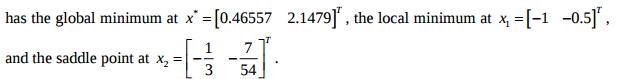
\includegraphics[width=0.7\linewidth]{screenshot002}
\label{fig:screenshot002}
\end{figure}


In general, the unconstrained nonlinear least squares problem is equivalent to:
\begin{flalign*}
\min_{x} \sum_{i=1}^N F_i^2(x)
\end{flalign*}
with the objective function:
\begin{flalign*}
f(x) = \frac{1}{2} \sum_{i=1}^N F_i^2(x)
\end{flalign*}

In the case of the following task, objective function will be
\begin{flalign*}
f(x) &= \frac{1}{2}(F_1^2 + F_2^2)\\
&= \frac{1}{2}[(x_1^6 + 6x_1^5 + 15x_1^4 - 2x_1^3x_2 + 18x_1^3 - 6x_1^2x_2 + 9x_1^2 - 6x_1x_2 + x_2^2)\\
&+\ \ \ 
(x_1^4 + 4x_1^3 - 2x_1^2x_2 + 6x_1^2 - 4x_1x_2 + 4x_1 + x_2^2 - 2x_2 + 1)]\\
&= \frac{1}{2}(x_1^6 + 6x_1^5 + 16x_1^4 - 2x_1^3x_2 + 22x_1^3 - 8x_1^2x_2 + 15x_1^2 - 10x_1x_2 + 4x_1 + 2x_2^2 - 2x_2 + 1)
\end{flalign*}
\\
And the point to check is:\\
\begin{math}
x = [x_1\ x_2]^T = [1\ 1]^T
\end{math}

The First order optimality condition is:\\
\begin{flalign*}
\nabla f(x^*) &= 0\\ \\
\frac{\delta f(x)}{\delta x_2} &= 400x_1^3 + 2x_1 -2 - 400x_2x_1\\
&= 400 + 2 - 2 - 400 = 0\\ \\
\frac{\delta f(x)}{\delta x_1} &= 200x_2 - 200x_1^2\\
&= 200 - 200 =  0
\end{flalign*}

In given point x = [1 1] the first--order optimality condition is fulfilled.

The Second order optimality condition is:\\
\begin{flalign*}
\nabla f(x^*) &= 0\ (calculated\ in\ previous\ step)\\ \and
\nabla^2 f(x^*)\ &= positive\ semi-definite\ matrix\\ \\
\nabla^2 f(x^*)\ &= 
\begin{bmatrix}%
\frac{\delta^2 f(x)}{\delta x_1^2} & \frac{\delta^2 f(x)}{\delta x_1x_2}\\
\frac{\delta^2 f(x)}{\delta x_1x_2} & \frac{\delta^2 f(x)}{\delta x_2^2}
\end{bmatrix}\\
&=
\begin{bmatrix}%
1200x_1^2 + 2 - 400x_2& - 400x_1\\
-400x_1& 200
\end{bmatrix}\\
for\ point\ [1\ 1] &=
\begin{bmatrix}%
1200 + 2 - 400& - 400\\
-400& 200
\end{bmatrix}\\
H &=
\begin{bmatrix}%
802& -400\\
-400& 200
\end{bmatrix}
\end{flalign*}
As it can be noticed, all principal minors are positive ($H_{1,1}\ and\ H_{2,2}$). Therefore the $H(x_*)$ is positive semi-definite.\\
\\
Octave code below was written to plot contour for this task.
\begin{lstlisting}
pkg load symbolic

syms x1 x2
f = @(x1,x2) 100.*(x2 - x1.^2).^2 + (1 - x1).^2;

ezcontour(f,[-3,3])
\end{lstlisting}

\begin{figure}[h]
\centering
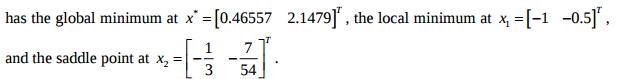
\includegraphics[width=0.7\linewidth]{screenshot002}
\caption{Contour plot of given function.}
\label{fig:screenshot002}
\end{figure}
\newpage

\clearpage
\chapter{Listings of algorithms}
\section{Coded selected algorithms}
Algorithm 1 - Simplex algorithm\\ 
\begin{lstlisting}

\end{lstlisting}
\newpage
Algorithm 2 - Revised Simplex algorithm\\
\begin{lstlisting}

\end{lstlisting}
\begin{thebibliography}{8}
\addcontentsline{toc}{chapter}{Bibliography}
%\addcontentsline{toc}{section}{Literatura}
\bibitem{nocedal}
J. Nocedal, S. J. Wright, Numerical Optimization, Springer, 1999,
\bibitem{zdunek}
Zdunek R., Optimization Methods - lecture slides.
\bibitem{mathworks}
Mathworks webpage, "Unconstrained Optimization Algorithms", https://www.mathworks.com/help/optim/ug/unconstrained-nonlinear-optimization-algorithms.html
\bibitem{uni}
Nonlinear Programming course webpage, North Carolina State University,
http://www4.ncsu.edu/~kksivara/ma706/
\end{thebibliography}

\end{document}

